\documentclass{article}
\author{Max Springenberg, 177792}
\title{
    DAP2 UB12\\
    Anja Rey, Gr.23 , Briefkasten 22
}
\date{}
\usepackage{amsmath}
\usepackage{amssymb}
\usepackage{stmaryrd}
\usepackage{graphicx}
\setcounter{section}{12}
% \Theta \Omega \omega
\newcommand{\tab}{\null \qquad}
\newcommand{\lA}{$\leftarrow$}
\newcommand{\ue}{$\infty$}

\begin{document}
\maketitle

\newpage
\subsection{Graphen}
\subsubsection \
Der Induktionsversuch ist falsch, da beispielsweise fuer n = 3 mit dem folgendem 
graphen:\\
%insert image
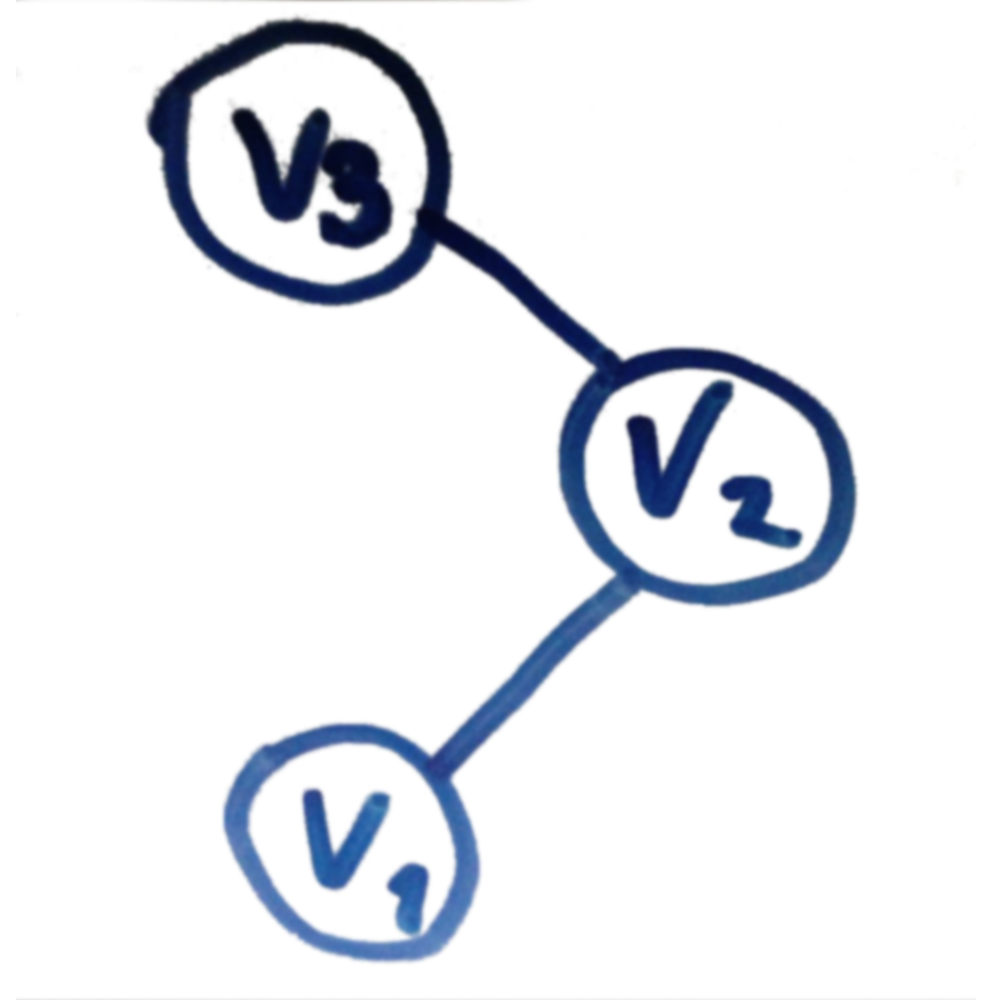
\includegraphics[height=5cm]{./1a.png}\\
\\
Beim entfernen des Knotens $v_2$ keine Kanten mehr vorhanden sind.\\
Somit ist der Induktionsschritt nicht fuer alle Knoten  geeignet.\\
\subsubsection \
Die Formel:\\
$$
\frac{'Knotenzahl' * ('Knotenzahl' - 1)}{2}
= \frac{|V| * (|V| - 1)}{2} = \frac{n * (n-1)}{2}
$$\\
gibt die maximale Kantenzahl an.\\
Ein Knoten kann mit den restlichen n-1 Knoten Kanten bilden. Jedoch gilt, dass die haelfte der Kanten doppelt 
gezaehlt werden, wenn man bedenkt, dass andere Knoten auch mit dem Knoten selbst wieder eine Kante bilden koennen.
Deshalb muss durch 2 dividiert werden.\\
\subsubsection \
Die Maximale Anzahl an Kanten kann mit der Formel aus 12.1.2 berechnet werden. Wir waehlen nun die minimale Anzahl loser
Knoten und die maximale Anzahl an Kanten fuer die verbleibenden Knoten.\\
\\
\begin{tabular}{ll}
    minimale lose Knoten & 1\\
    Anzahl verbleibender Knoten & n - 1\\
\end{tabular}\\
\\
wir setzen nun also fuer n, n - 1 in die Formel ein. 
Daraus resultiert die maximale Kantenzahl: $\frac{(n-1) * (n-2)}{2}$\\

\newpage
\subsection{Algorithmus von Dijkstra}
\subsubsection \
\begin{tabular}{l|l|l|l|l|l}
         & a&  b&  c&  d&  e\\
    \hline
    d    & 0&\ue&\ue&\ue&\ue\\
    color& w&  w&  w&  w&  w\\
\end{tabular}\\
$u = a$\\
$Q=\{(a, 1), (b, \infty), (c, \infty), (d, \infty), (e, \infty)\}$\\
\\
\begin{tabular}{l|l|l|l|l|l}
    \hline
         &  a&  b&  c&  d&  e\\
    \hline
    d    &  0&  4&\ue&  1& 12\\
    color&  s&  w&  w&  s&  w\\
\end{tabular}\\
$u = d$\\
$Q=\{(d, 1), (b, 4), (e, 12), (c, \infty)\}$\\
\\
\begin{tabular}{l|l|l|l|l|l}
    \hline
         &  a&  b&  c&  d&  e\\
    \hline
    d    &  0&  4& 14&  1&  2\\
    color&  s&  w&  w&  s&  s\\
\end{tabular}\\
$u = e$\\
$Q=\{(b, 4), (d, 14)\}$\\
\\
\begin{tabular}{l|l|l|l|l|l}
    \hline
         &  a&  b&  c&  d&  e\\
    \hline
    d    &  0&  4&  6&  1&  2\\
    color&  s&  s&  w&  s&  s\\
\end{tabular}\\
$u = b$\\
$Q=\{(c, 4)\}$\\
\\
\begin{tabular}{l|l|l|l|l|l}
    \hline
         &  a&  b&  c&  d&  e\\
    \hline
    d    &  0&  4&  6&  1&  2\\
    color&  s&  s&  s&  s&  s\\
\end{tabular}\\
$u = c$\\
$Q=\emptyset$\\
\\

\subsubsection \
Die Heap-Eigenschaft eines AVL-Baumes wieder her zu stellen benoetigt O(log(n)), wir muessen unsere Liste immer wieder
neu sortieren und landen damit in O(n*log(n)).

\end{document}
